\section{Architettura}

Per l'architettura dell'applicativo da sviluppare si è deciso di utilizzare \textit{Model-View-ViewModel}, derivato da \textit{Model-View-Controller}.

\subsection{Diagrammi dei package}
\subsection{Diagrammi delle classi}

\subsubsection{View}

\begin{figure}[h!]
    \centering
    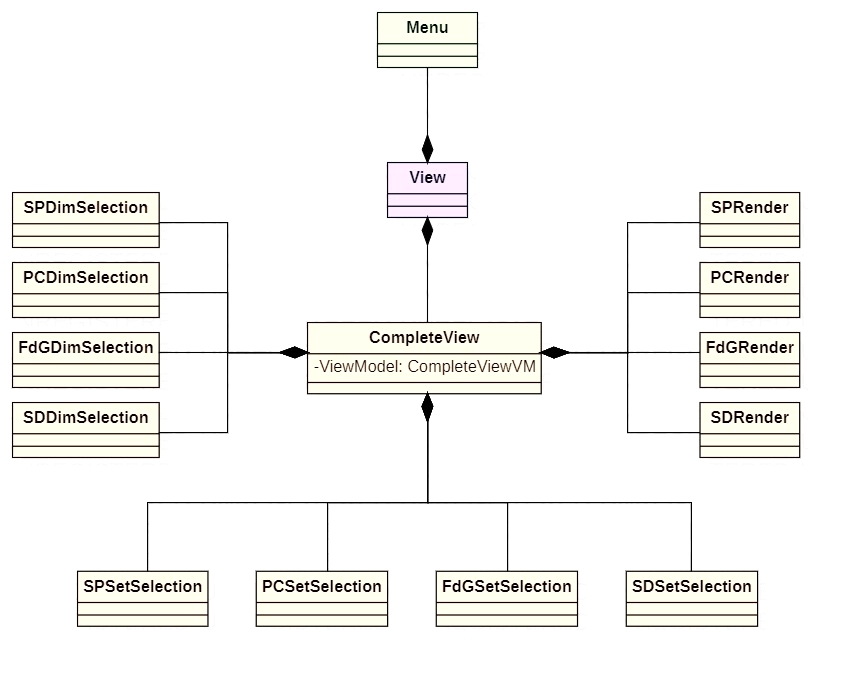
\includegraphics[scale=0.75]{../../assets/classi_uml/View.jpg}
    \caption{Diagramma delle classi - View}
\end{figure}
\newpage
\subsubsection{Model}

\begin{figure}[h!]
    \centering
    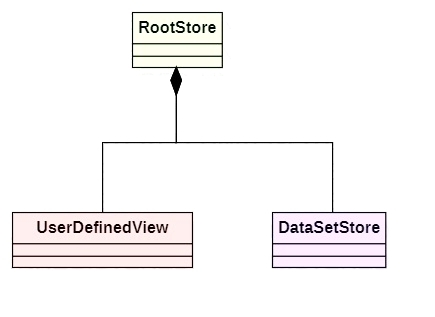
\includegraphics[scale=0.75]{../../assets/classi_uml/Model.jpg}
    \caption{Diagramma delle classi - Model}
\end{figure}

\subsection{Diagrammi di sequenza}